Let $G=(V,E)$ be an unweighted graph and $\mathcal{G}$ a graph drawn uniformly at random from all possible graphs with the same vertex set $V$ and exactly $m$ edges. For a partition $\zeta$, the probability that $\mathcal{G}$ has at least $m_\zeta$ intracluster edges and $p_\zeta$ intracluster pairs is modeled after the inverse cumulative hypergeometric distribution, $\Pr( m_\zeta \leq m)$:
\begin{equation}\label{eq:surprise}
S(\zeta) := \sum_{i = m_\zeta}^m \dfrac{\binom{p_\zeta}{i} \binom{p-p_\zeta}{m-i} }{\binom{p}{m}} = 1- \sum_{i = 0}^{m_\zeta} \dfrac{\binom{p_\zeta}{i} \binom{p-p_\zeta}{m-i} }{\binom{p}{m}}.
\end{equation}

Surprise computes the probability to (surprisingly) observe at least as many internal edges as within the proposed partition in a uniform random graph. Model in Eq. \ref{eq:surprise}  corresponds to an urn model without reinsertion, where $S$ is the probability of extracting at least $m_\zeta$ white balls out of $m$ trials from an urn containing $p_\zeta$ white balls and $p-p_\zeta$ black balls. It's worth noting that $S$ is $p$-value of a one-tailed Fisher exact-test where one is asking how confidently should reject the null hypothesis that the intracluster density is the same as the graph density (see further section~\ref{sec:surprisefishertest}). Intuitively, the lower $S(\zeta)$, the better the clustering. Optimal partitions with respect to $S$ are those with the highest number of intracluster edges and the smallest number of intracluster pairs.

It should be noted that due to numerical precision problems in the evaluation of large binomial coefficients, $\hat{S}(\zeta) := -\log_{10}S(\zeta)$ is often taken as measure of quality of the partition, with higher values corresponding to better clustering. Different authors \cite{ArnauVMarsS2005}, \cite{Fleck2014} refer to $S$ as Surprise, whereas others \cite{Aldecoa2011}, \cite{Aldecoa2013} use $\hat{S}$. Hereafter we stick to the notation of \cite{Fleck2014} where Surprise is indicated as $S$ defined in Eq. \ref{eq:surprise}.

As noted by \cite{Fleck2014}, for a given graph, $m$ and $p$ are fixed so $S(\zeta)$ depends only on number of intracluster edges $m_\zeta$ and intracluster pairs $p_\zeta$, namely on the clustering $\zeta$. The landscape of this two-variables function can be explored with the help of the urn model. A clustering $\zeta$ must satisfy the following (intuitive but important) properties:
\begin{enumerate}\label{list:urn_model_properties}
\item $0 \leq m_\zeta \leq p_\zeta$\\It's impossible to draw more white balls than the white balls contained in the urn.
\item $m\geq m_\zeta$\\It's impossible to have more white balls than total number of drawn balls.
\item $p-p_\zeta \geq m-m_\zeta$\\It's impossible to draw more black balls than the black balls contained in the urn.
\end{enumerate}
The urn model also helps us to figure out some of the extremely important properties of $S$ that we'll refer in the next sections of this work:
\begin{description}
\item[(i)]\label{list:surprise_properties} It's less probable to have at least $m_\zeta+1$ than $m_\zeta$ white balls drawn if the urn contains the same number of $p_\zeta$ white balls:
$$S(m_\zeta+1,p_\zeta) < S(m_\zeta,p_\zeta).$$
\item[(ii)] It's less probable to have at least $m_\zeta$ white balls drawn if the urn has one white balls less: if $m_\zeta >0$ then $$S(m_\zeta,p_\zeta-1) < S(m_\zeta,p_\zeta).$$
\item[(iii)] It's less probable to have at least $m_\zeta+1$ white balls drawn from an urn with one white balls more than from having at least $m_\zeta$ white balls from an urn with $p_\zeta$ white balls). If $p-p_\zeta> m-m_\zeta$ then $$S(m_\zeta+1,p_\zeta+1) < S(m_\zeta,p_\zeta).$$
\end{description}
The scheme in Figure \ref{fig:surprisebehaviour} explicits the order relation between the elements of the three aforementioned inequalities.
\begin{figure}[htb]
\centering
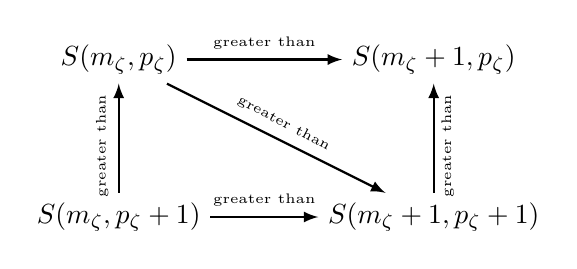
\begin{tikzpicture}
    \node[] (S00) at (0,0) {$S(m_\zeta,p_\zeta)$};
    \node[] (S10) at (4,0) {$S(m_\zeta+1,p_\zeta)$};
    \node[] (S01)  at (0,-2) {$S(m_\zeta,p_\zeta+1)$};
    \node[] (S11)  at (4,-2) {$S(m_\zeta+1,p_\zeta+1)$};
    
    \draw[->,thick,>=latex] (S00) -- node[anchor=south] {\tiny{greater than}} (S10);
    \draw[->,thick,>=latex] (S01) -- node[anchor=south] {\tiny{greater than}} (S11);
    \draw[->,thick,>=latex] (S11) -- node[anchor=west,xshift=5,yshift=-25,rotate=90] {\tiny{greater than}} (S10);

    \draw[->, thick,>=latex] (S00) -- node[anchor=south,rotate=-28] {\tiny{greater than}} (S11);
    \draw[->,thick,>=latex] (S01) -- node[anchor=west,xshift=-6,yshift=-25,rotate=90] {\tiny{greater than}} (S00);
\end{tikzpicture}
\caption{Behaviour of the landscape of Surprise $S$.}
\label{fig:surprisebehaviour}
\end{figure}

A fourth inequality $S(m_\zeta,p_\zeta+1)>S(m_\zeta+1,p_\zeta)$ is implicit by looking at the behaviour of $S(\zeta)$ for a given graph. The scheme in Figure \ref{fig:surprisebehaviour} allows to rank the values of Surprise in relation to changes in $m_\zeta$ and $p_\zeta$, in particular, it's easy to verify that $S$ satisfies the following strict order relation:
\begin{equation}\label{eq:surpriseorderrelation}
S(m_\zeta+1,p_\zeta)<S(m_\zeta+1,p_\zeta+1)<S(m_\zeta,p_\zeta)<S(m_\zeta,p_\zeta+1).
\end{equation}

In the convex interval $\mathcal{L}$ such that:
\begin{equation}
\mathcal{L} := \{ ( m_\zeta,p_\zeta) \; | m_\zeta > 0 \land p_\zeta \geq m_\zeta \land m \geq m_\zeta \land p-m > p_\zeta - m_\zeta \}
\end{equation}
Surprise is a monotonically increasing (decreasing $\hat{S}$) function of $p_\zeta$ and monotonically increasing function of $m_\zeta$ (increasing $\hat{S}$) as shown in Figure~\ref{fig:monotonical_surprise}.


\begin{figure}[htb]
\centering
\begin{tikzpicture}[scale=0.6, every node/.style={scale=0.6}]
\def \S {1};
\def \W {11};
\def \H {7};
\node[anchor=south west, inner sep=0mm] at (0,0) { \includegraphics[width=\W cm]{images/plot_surprise_pareto.pdf}};
\node[anchor=south] at (\W /2,\H +0.25) {$S(m_\zeta,p_\zeta$, $m=5$,$p=15$)};
%\draw[help lines,xstep=1.0,ystep=1.0] (0,0) grid (\W,\H);
\foreach \x in {1,...,\W } {\node [anchor=north] at (\x-0.5,0) {$\x$}; }
\node[anchor=north] at (\W/2,-0.5){$p_\zeta$};
\foreach \y in {1,...,\H} {\node [anchor=east] at (0 ,\y-0.5) {$\y$}; }
\node[anchor=east] at (-0.5,\H/2){$m_\zeta$};
%\node[rectangle,fill=black!10,draw=black,rounded corners=0.1cm] at (\W+1.5,\H-0.5) {$m_{\zeta},p_\zeta \not \subset \mathcal{L}$};
\end{tikzpicture}
\caption{Surprise increases as it gets hotter. The grey area is outside the domain of validity $\mathcal{L}$ while white are $S=0$.}
\label{fig:monotonical_surprise}
\end{figure}

Moreover, from Figure \ref{fig:surprisebehaviour} and Figure ~\ref{fig:monotonical_surprise} follows that an optimal solution with respect to $S$ is pareto-optimal with respect to maximizing $m_\zeta$ and minimizing $p_\zeta$.

With the tools of \ref{eq:surpriseorderrelation} in mind, one can infere how Surprise behaves under a perturbation of $m_\zeta$ and $p_\zeta$ by some amount $(\delta_{m_\zeta},\delta_{p_\zeta})$ and obtain a very useful tool that will help us in the rest of this work:
\begin{equation}\label{eq:resolution_limit_condition}
S(m_\zeta + \delta_{m_\zeta}, p_\zeta + \delta_{p_\zeta}) < S(m_\zeta,p_\zeta) \iff \delta_{m_\zeta} \geq \delta_{p_\zeta}
\end{equation}

The result in Eq.\ref{eq:resolution_limit_condition} is of great help in designing optimization algorithms as every move that increase the intracluster edges more than intracluster pairs is good, while moves that increase intracluster pairs more than intracluster edges must be ignored, therefore sparing time for the computation of Surprise. Additionally, Eq.\ref{eq:resolution_limit_condition} is a useful when analyzing the onset of the resolution limit for different models.
In the next sections we will also cast light on resolution limit for Surprise, to show with convincing theoretical arguments that $S$ is nearly resolution-limit-free in Traag's sense~\cite{traag2015}.

\section{Surprise is a statistic test}\label{sec:surprisefishertest}
It should be noted that \emph{Surprise} is the p-value of the one-tailed Fisher exact test. In particular one can draw the contingency table for the urn model as:

\begin{table}[htb]
\centering
\begin{tabular}{|c|c|c|c|}
\hline
 & Drawn & Not drawn & \textbf{Total}\\
\hline
Intracluster & $m_\zeta$ & $p_\zeta-m_\zeta$ & $p_\zeta$\\
\hline
Intercluster & $m-m_\zeta$ & $p-m-p_\zeta+m_\zeta$ & $p-p_\zeta$ \\
\hline
\textbf{Total} & $m$ & $p-m$ & $p$ \\
\hline
\end{tabular}
\end{table}
The odds-ratio $\textrm{OR} \in (0,\infty)$ of this $2\times 2$ contingency table is
\begin{equation}
\textrm{OR} = \frac{m_\zeta(p-m-p_\zeta+m_\zeta)}{(m-m_\zeta)(p_\zeta-m_\zeta)} 
\end{equation}
In particular minimizing Surprise corresponds to maximizing the odds-ratio $\textrm{OR}$. Very low values of $S$ tells us that we can reject the null hypothesis $H_0 := \textrm{OR} \neq 1$ with high probability.

It can be shown that when the entries of the contingency table are big enough, computing $S$ corresponds to computing the $\chi^2$ statistic and it is also possible to tackle the problem of computation of $S$ by means of odds-ratio.
If one computes the \emph{normalized log odds-ratio}:
\begin{equation}
\log(\textrm{OR}) = \log\left( \frac{m_\zeta(p-m-p_\zeta+m_\zeta)}{(m-m_\zeta)(p_\zeta-m_\zeta)} \right )
\end{equation}
and seeks the probability
\begin{equation}
\Pr\left(z < -\frac{|\log\textrm{OR})|}{SE} \right)
\end{equation}
where $z$ is a random variable with standard normal distribution $z \approx \mathcal{N}(0,1)$.